\section{Background}\label{sec:background}

In this section we will present the necessary background information to follow our implementation of the \textit{Normalized convolution} domain transform filtering algorithm. For a more detailed explanation of the method and its theoretical background, please refer to the original paper~\cite{GastalOliveira2011DomainTransform}.

The general outline of the algorithm is given in Figure~\ref{flowchart}. We distinguish two algorithm steps. First is the initialisation step, when the domain transform data of the image is computed and stored. Second is the filtering step, when multiple filter iterations are applied to the image data using the domain transform information.

\subsection{Domain transform}
The straightforward approach to image blurring is to compute a new value for each image pixel using the weighted average of its neighbourhood. To decide whether a pixel lies in this neighbourhood, some distance measure is necessary. In the case of simple edge unaware blurring (such as applying a Gaussian filter) this distance measure is the spatial distance between image pixels. However to achieve edge-aware image filtering the radiometric distance between pixels (their difference in color) has to be taken into account as well. In general this increases the dimensionality of the problem by adding a dimension for each colour channel.

For a RGB color image this would lead to a 5-dimensional space (3 radiometric + 2 spatial dimensions). The domain transform method reduces this dimensionality as follows.
Firstly, it treats the two spatial dimensions separately, which means that the image is successively filtered along its rows and columns separately. Secondly, it merges the three radiometric dimensions and the remaining one spatial dimension into the one-dimensional space of the domain transform. This transformation retains the necessary distance properties from the original space.

Looking at a single image row, the pixels can be enumerated from left to right as $ p_0 \dots p_n$. Each pixel $p_i$ is associated with a domain transform value $dt_i$, and it holds that $\forall k : dt_k \leq dt_{k+1}$. In other words, the series of domain transform values is monotonically increasing. The exact difference between two consecutive domain transform values depends on the spatial and radiometric distance between pixels.

This data is computed and stored for all image rows and all image columns.

\subsection{Filtering iterations}

For the filtering step, multiple (usually three) filtering iterations are applied to the image. Each iteration consists of filtering along all rows and then filtering along all columns.

Filtering happens using a box filter. This means that a pixels new value is the uniform average of the pixels in its neighbourhood. For a single pixel $p_i$ this neighbourhood consists of all pixels $p_k$ for which it both holds that $dt_k < dt_i+r$ and $dt_k > dt_i-r$, where $r$ is the filtering radius that changes from iteration to iteration. The size of this neighbourhood can vary significantly between pixels and strongly depends on the input image.

The use of a box filter might first look like a severe restriction as usually a Gaussian filter response is preferable. However the multiple consecutive iterations of box filtering in fact produce a Gaussian like filtering response.

\subsection{Cost Analysis}
In asymptotic terms, the algorithm has a complexity of \BigO{n}, which makes it already very competitive with other approaches to edge-aware image filtering. For optimization purposes we are however interested in a more thorough cost analysis of the method. Therefore we have counted the number of different floating point operations executed by the implementation, the numbers can be seen in Table~\ref{cost_analysis}. These numbers were used for performance computations and analysis in the course of optimisation.

The following variables are used in Table~\ref{cost_analysis}: $W$ - width of the processed image, $H$ - height of the processed image, $N$ - number of filtering iteration. \\ \lstinline{TransformedDomainBoxFilter} is the filtering function which executes one pass through the image in one direction. \lstinline{Filter} is the main method called on the whole image. It includes all necessary precomputation and multiple iterations of the filter itself.

\begin{table}[h]
\label{cost_analysis}
\centering
\begin{tabular}{| l | p{3cm} | p{3cm} |} \hline 
Operation & TransformedDomain BoxFilter  & Filter \\ \hline
add & $2 \cdot N \cdot 4HW$ & $(8 + 8N)HW$ \\ \hline
subtract & $2 \cdot N \cdot 4HW$ & $(6 + 8N)HW$ \\ \hline
compare & $2 \cdot  N \cdot 4HW$ & $(8N)HW$ \\ \hline
multiply & $2 \cdot N \cdot 3HW$ & $(2 + 6N)HW + 3N$ \\ \hline
divide & $2 \cdot N \cdot HW$ & $(2HW + 1)N + 1$ \\ \hline
fabs & $0$ & $6HW$ \\ \hline
sqrt & $0$ & $3N$ \\ \hline
powf  & $0$ & $2N$ \\ \hline
\end{tabular}
\caption{Floating point operations performed in the code}
\end{table}

\begin{figure}\vspace{-1mm}
  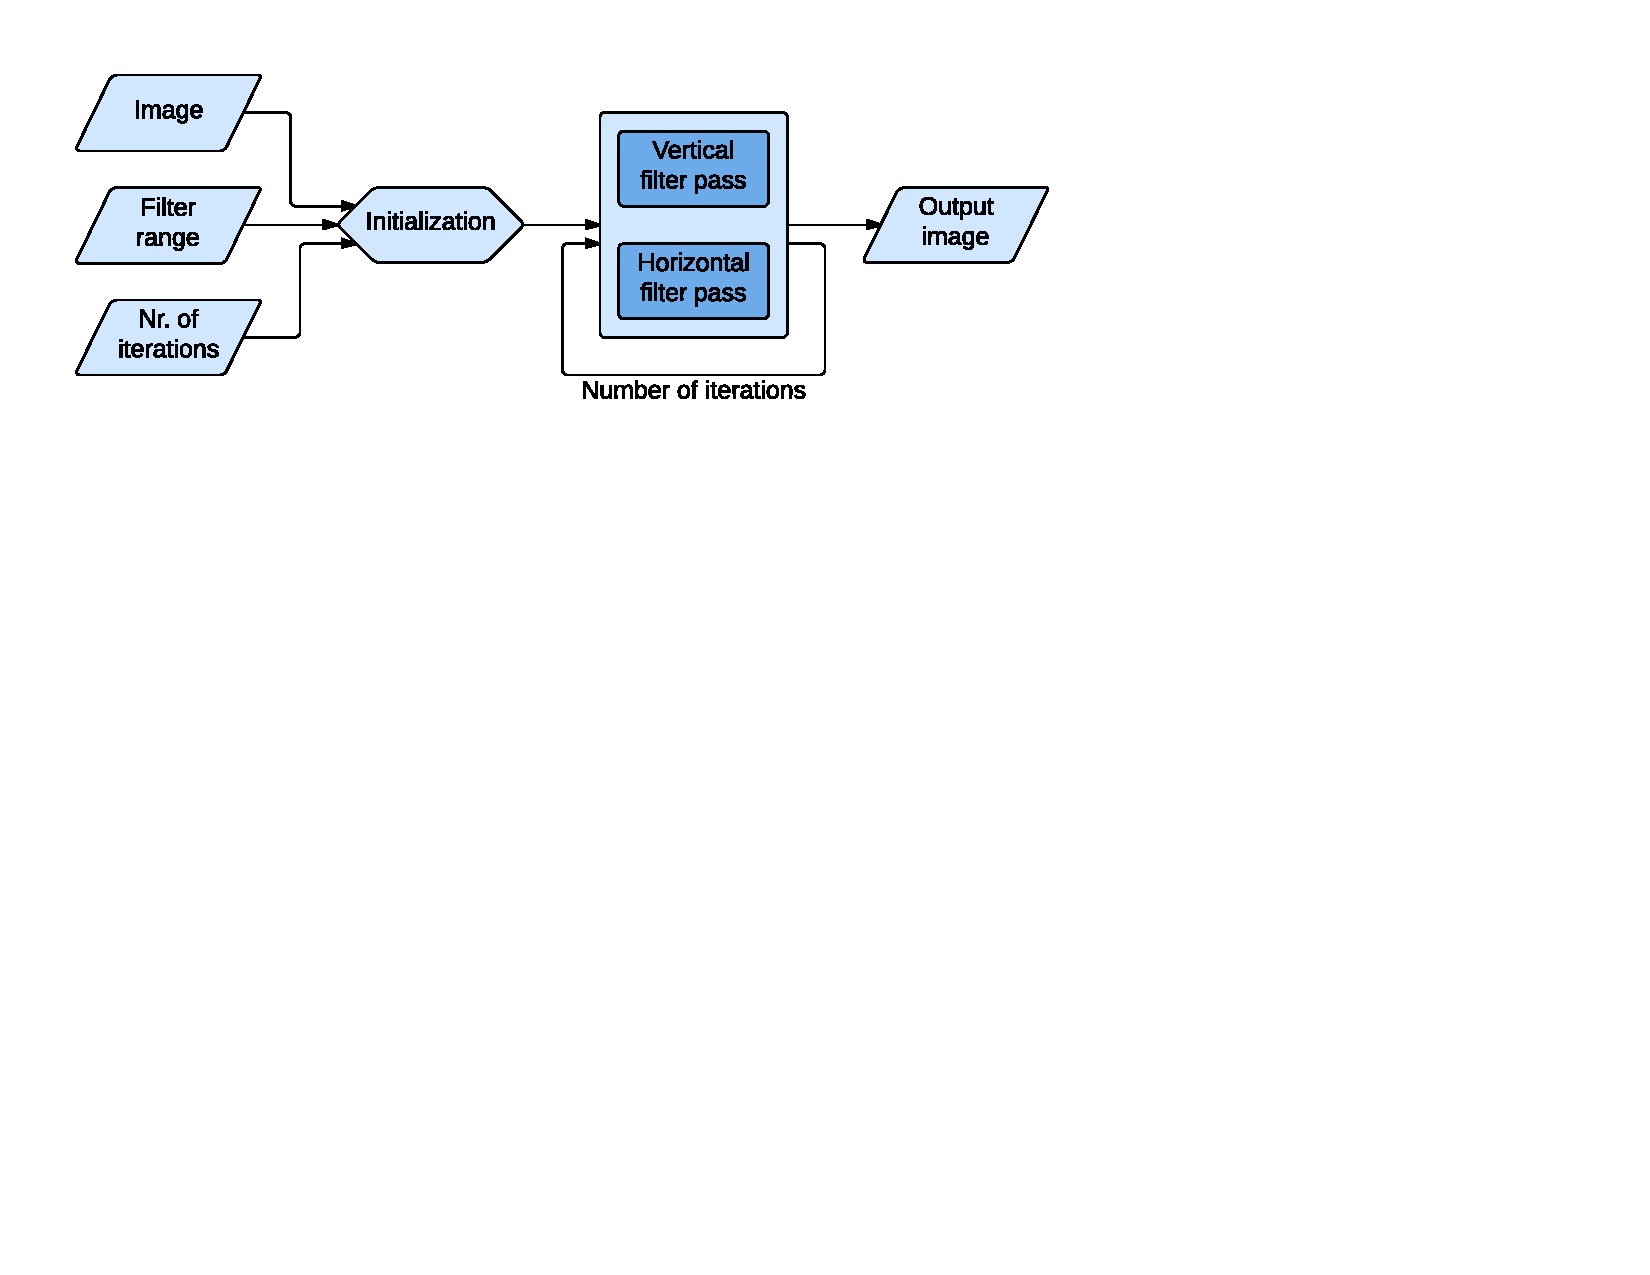
\includegraphics[trim=10mm 145mm 100mm 10mm, clip, width=0.48\textwidth]{figures/flowchart.pdf}
  \caption{Algorithm flowchart\label{flowchart}}
\end{figure}

\comment{
Give a short, self-contained summary of necessary
background information. For example, assume you present an
implementation of FFT algorithms. You could organize into DFT
definition, FFTs considered, and cost analysis. The goal of the
background section is to make the paper self-contained for an audience
as large as possible. As in every section
you start with a very brief overview of the section. Here it could be as follows: In this section 
we formally define the discrete Fourier transform, introduce the algorithms we use
and perform a cost analysis.

\mypar{Discrete Fourier Transform}
Precisely define the transform so I understand it even if I have never
seen it before.

\mypar{Fast Fourier Transforms}
Explain the algorithm you use.

\mypar{Cost Analysis}
First define you cost measure (what you count) and then compute the
cost. Ideally precisely, at least asymptotically. In the latter case you will need to instrument your code to count
the operations so you can create a performance plot.

Also state what is
known about the complexity (asymptotic usually) 
about your problem (including citations).

Don't talk about "the complexity of the algorithm.'' It's incorrect,
remember (Lecture 2)?
}